%
%	Documento de análisis y diseño
%

\documentclass[11pt, a4paper, twoside, titlepage]{article}
\usepackage[utf8x]{inputenc}
\usepackage[T1]{fontenc}
\usepackage[spanish, es-ucroman]{babel}
\usepackage{lmodern}
\usepackage{anysize}
\usepackage{fancyhdr}
\usepackage[none]{hyphenat}
\usepackage[colorlinks, linkcolor=red]{hyperref}
\usepackage{float}
\usepackage{lscape}
\usepackage{pdflscape}
\usepackage[doc=anaydis]{isdiedral}

% Nombre del documento (para futuras referencias)
\newcommand*{\doctitle}{Análisis y diseño}
\newcommand*{\docversion}{1.0}


%%% Configuraciones %%%
\marginsize{2.5cm}{2cm}{2cm}{2cm}

% Usa como familia tipográfica por defecto "Sans"
\renewcommand{\familydefault}{\sfdefault}

% Establece la profundidad hasta la cual se numeran los elementos de sección
\setcounter{secnumdepth}{4}

% Establece la profundidad de niveles de sección que aparece en el TOC
\setcounter{tocdepth}{4}

% Configuración de los encabezados
\encabezadodiedral{\doctitle{} \docversion}
\pagestyle{fancy}

\renewcommand*{\thepage}{\sffamily \roman{page}}

\title{\doctitle\\\textsl{Airline Common Environment}}
\author{Grupo Diedral}

% Metadatos del pdf
\hypersetup{
pdfinfo={
	Author={Grupo Diedral},
	Title={\doctitle{} \docversion},
	Subject={Airline Common Environment},
	Keywords={análisis, diseño,  UML, Airline Common Environment, Ingeniería del Software}
}
}

\begin{document}
	% Tabla de cambios
	\begin{tablacambios}
		1.0 & 31 de mayo de 2013 & Todos & Versión inicial
	\end{tablacambios}

	% Cita inicial
	\fijacitainicial{Hay dos formas de elaborar un diseño software: una es hacerlo simple para que sea obvio que no hay deficiencias, la otra es hacerlo suficientemente complicado para que no haya deficiencias obvias. El primer método es mucho más difícil}{C.A.R. Hoare (1980)}

	% Portada
	\portadaace{\doctitle}{\docversion}

	\tableofcontents
	\newpage

	\iniciarnumeraciondiedral

	\parskip = .2cm

	% -- Introducción
	\section{Introducción}
		\subsection{Propósito}
			Este documento recoge la documentación generada durante las fases de análisis y diseño del módulo de \textit{Gestión Externa} del proyecto de Ingeniería del Software \textit{Airline Common Environment}.

			En primer lugar se incluye la parte correspondiente al análisis de requisitos que recoge el diagrama de modelo de dominio, en el que se presentan y relacionan los conceptos generales procedentes del dominio del producto; y los diagramas de actividad, que enuncian el flujo de comportamiento de los casos de uso.

			La siguiente sección del documento desarrolla los diagramas generados durante la fase de análisis: el diagrama de paquetes, el diagrama de clases de análisis y los diferentes diagramas de comunicación correspondientes a cada caso de uso.

			Finalmente se incluye la documentación de diseño que comprende los diagramas de secuencia y el diagrama de clases de diseño junto con epígrafes explicativos del diseño y los patrones empleados.


		Esta información ha sido especificada por medio del {\itshape Lenguaje Unificado de Modelado} (UML).

		\paragraph*{Nota sobre herramientas empleadas:} para la elaboración de los diagramas se ha utilizado el\break programa {\normalfont BoUML} en su versión {\normalfont 4.23 patch 7 `ultimate'}.


	% -- Requisitos
	\section{Requisitos}
		\subsection{Modelo de dominio}
				\begin{center}
					\hspace*{-.5cm}
					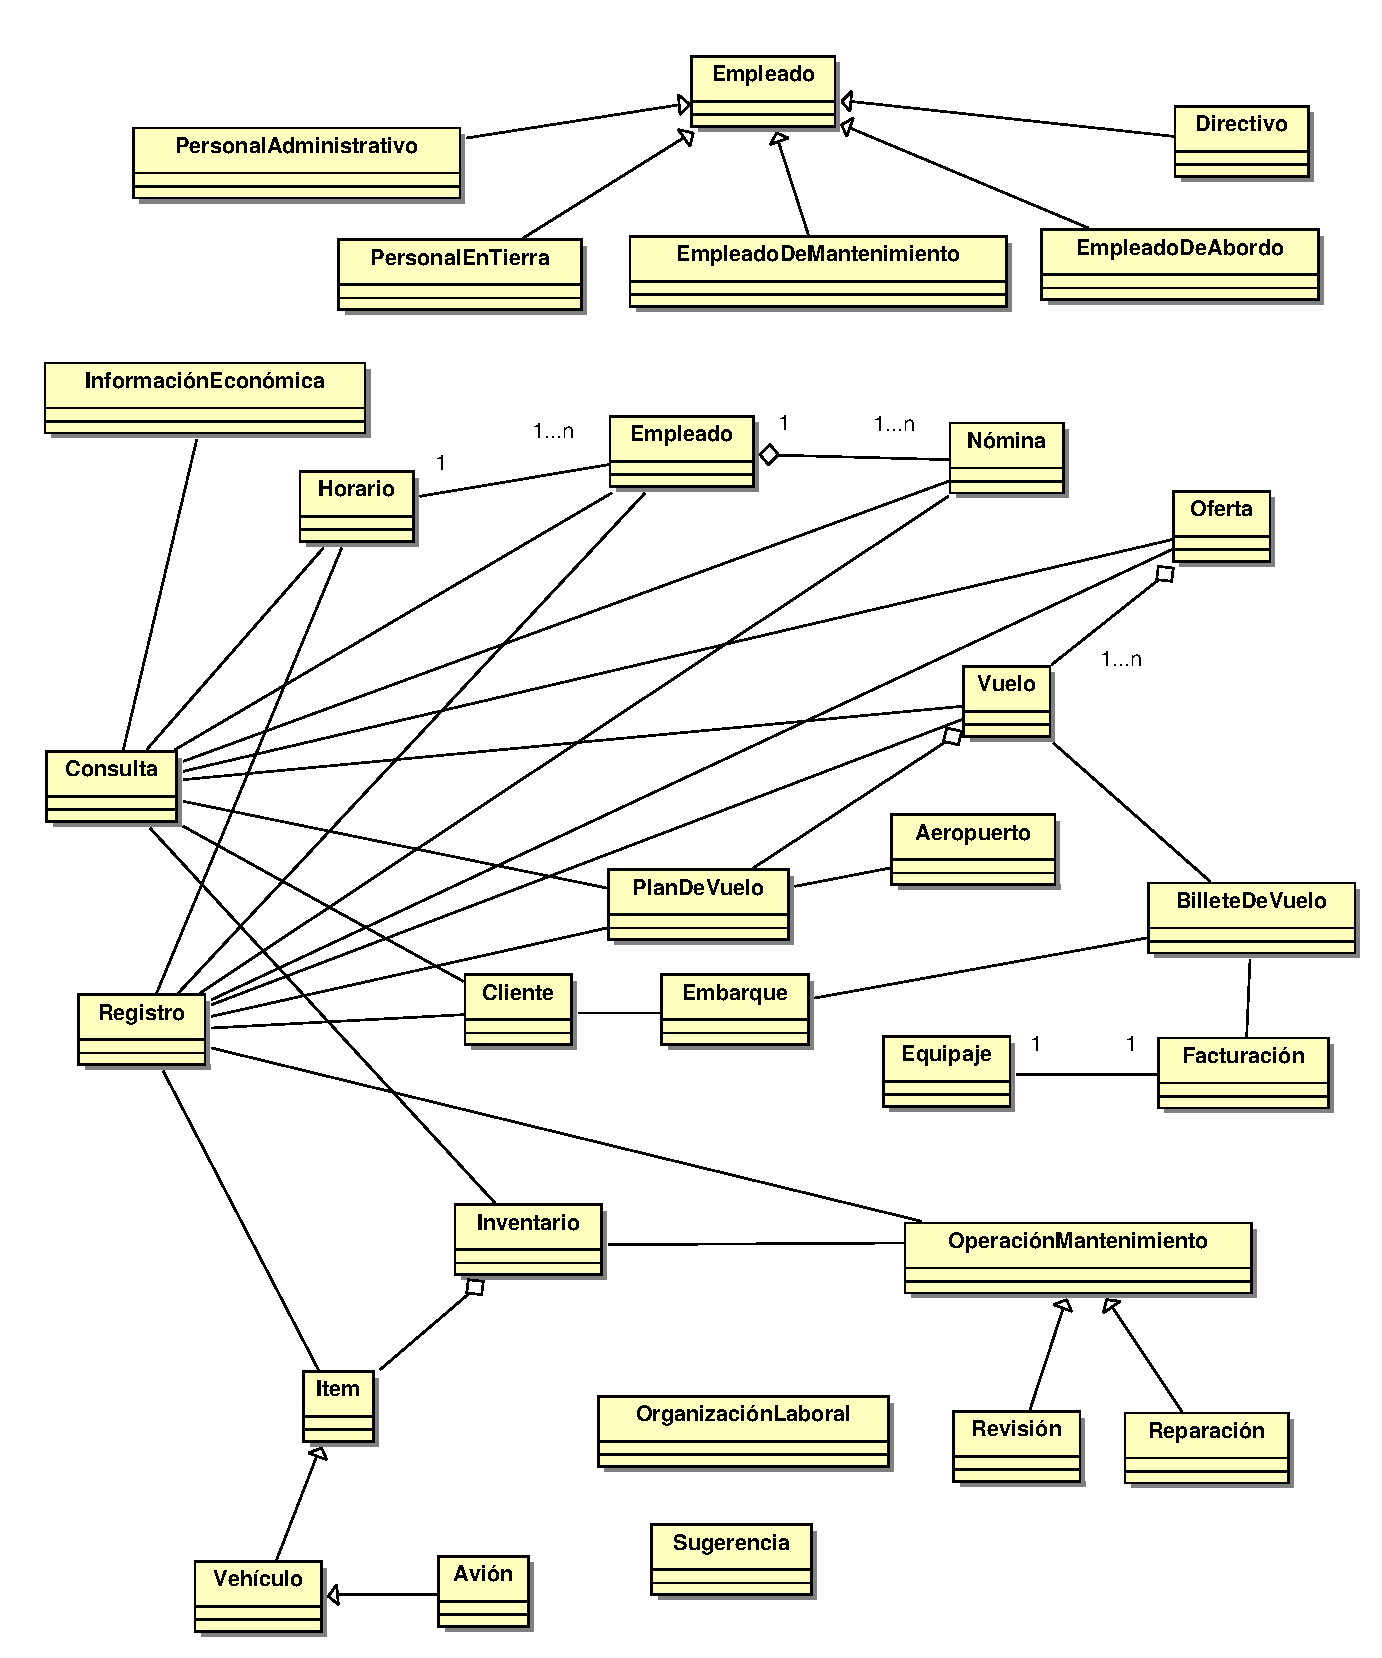
\includegraphics[scale=.722]{analisis/diagramas/modelodominio.pdf}
				\end{center}	
			\newpage
		\subsection{Diagramas de actividad}
			\subsubsection{Acceder web}
				\begin{center}
					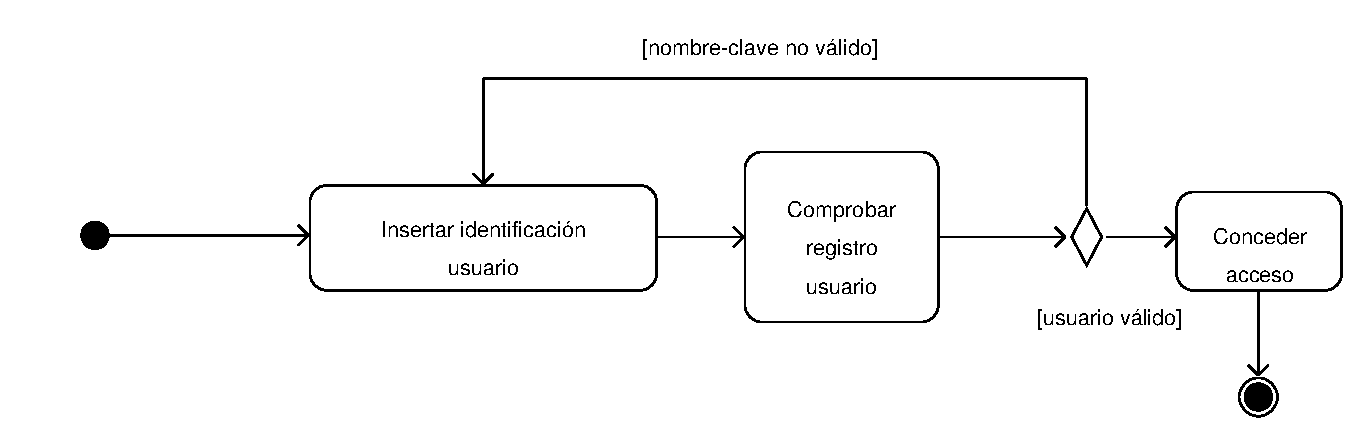
\includegraphics[scale=.67]{analisis/diagramas/da_accederweb.pdf}
				\end{center}

				Para acceder a la web, el usuario introduce sus datos identificativos, se comprueba la validez de éstos y si son válidos, el usuario se considera identificado lo que le concede acceso a las funcionalidades de la aplicación que así lo requieran. En caso de que los datos sean erróneos se advierte al usuario de ello y vuelve a la inserción de datos.

			\subsubsection{Comprar billete}
				\begin{center}
					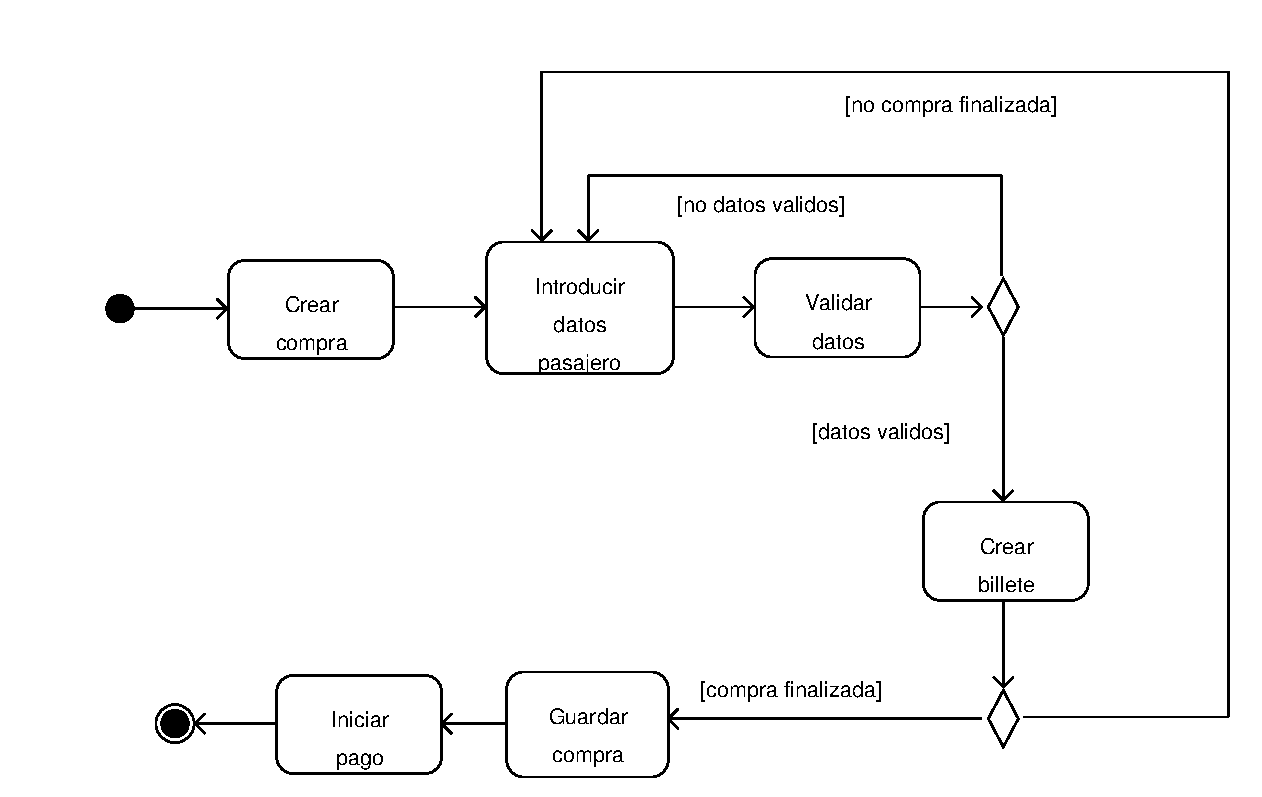
\includegraphics[scale=.72]{analisis/diagramas/da_comprarbillete.pdf}
				\end{center}
				El caso de uso {\itshape Comprar billete} empieza creando una compra y termina iniciando el pago correspondiente a dicha compra.
				El usuario debe empezar introduciendo los datos del pasajero, y aqui se bifurca en dos caminos. Si los datos no son válidos, volvemos a la secuencia de introducir datos. Si los datos son válidos, se crea un nuevo billete y volvemos a tener dos opciones. Si la compra no ha seguido el proceso de ser finalizada, volvemos de nuevo a la posibilidad de introducir los datos del pasajero. Sin embargo, si se sigue por el proceso de compra finalizada, se guarda la compra y se inicia su pago.

			\subsubsection{Consultar oferta}
				\begin{center}
					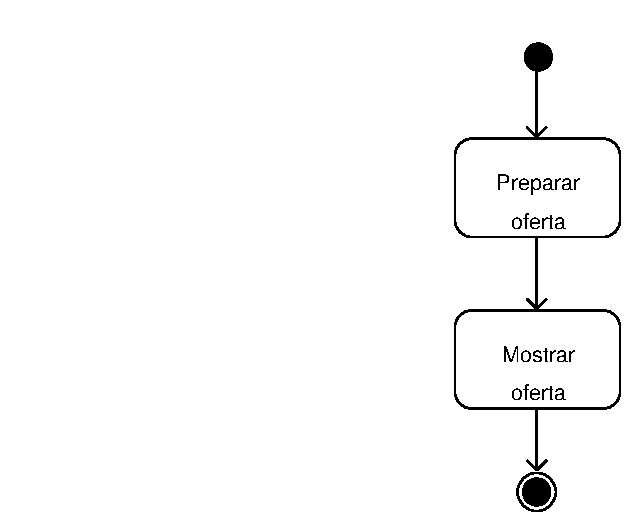
\includegraphics[scale=.7]{analisis/diagramas/da_consultaroferta.pdf}
				\end{center}
				El caso de uso {\itshape Consultar oferta} se encarga de mostrar una oferta ya seleccionada por el usuario. 
				
				Debido a que el flujo de pago es único, el sistema procede al preparar los datos de la oferta que le ha sido envidada y posteriormente la muestra por pantalla.

			\subsubsection{Consultar vuelos}
				\begin{center}
					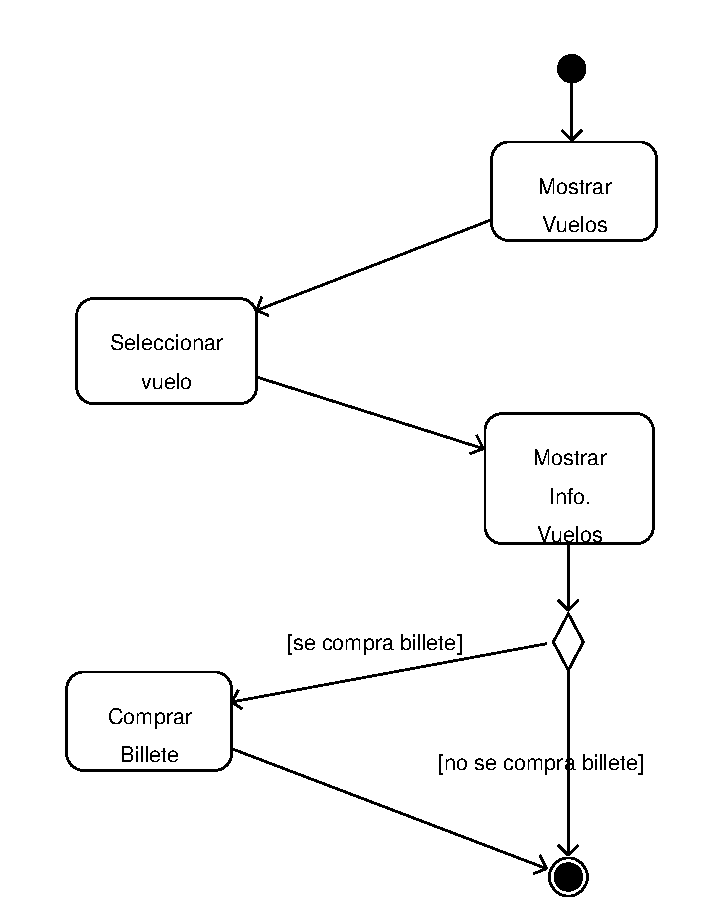
\includegraphics[scale=.71]{analisis/diagramas/da_consultarvuelos.pdf}
				\end{center}
				El caso de uso {\itshape Consultar vuelos} permite mostrar los vuelos para que el usuario los visualice y por otra parte conectar los vuelos con la compra del billete  de un vuelo concreto.
				Primero se muestran todos los vuelos disponibles en el sistema, el usuario selecciona un vuelo concreto y se muestra la información de ese vuelo. Posteriormente, se bifurcan dos caminos. Se puede realizar la compra de un billete y redireccionar al proceso de dicha compra, o en caso contrario se finalizará directamente el caso de uso.
			\subsubsection{Editar datos personales}
				\begin{center}
					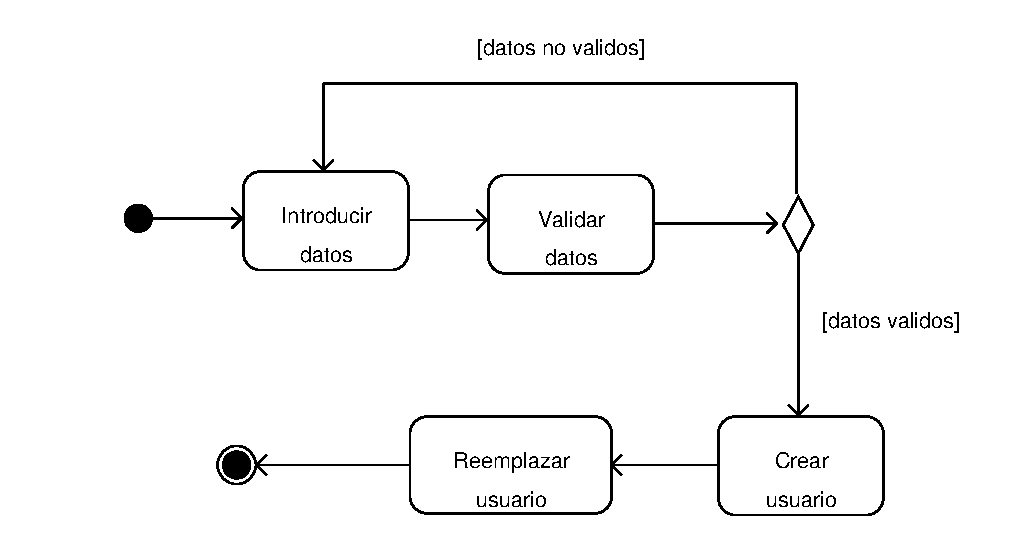
\includegraphics[scale=.86]{analisis/diagramas/da_editardatospersonales.pdf}
				\end{center}
				El caso de uso {\itshape Editar datos personales} permite que un usuario con una sesion iniciada edite sus datos personales (nombre, apellidos, direccion de correo electrónico asociada y modificar la contraseña con sus métodos de seguridad correspondientes para ello). 
				La secuencia empieza cuando el usuario introduce los datos a modificar y esos se validan. En este punto, si los datos no son válidos se vuelve a pedir al usuario que introduzca los datos de nuevo. Si son válidos, se crea un nuevo usuario la mezcla de datos modificados y antiguos, y se reemplaza por el ya existente en el sistema (el usuario no se modificará directamente para evitar romper las barreras de abstracción de los lenguajes orientados a objetos y trae menos problemas con los TADS empleados en el almacenamiento de usuarios).

			\subsubsection{Iniciar pago billetes}
				\begin{center}
					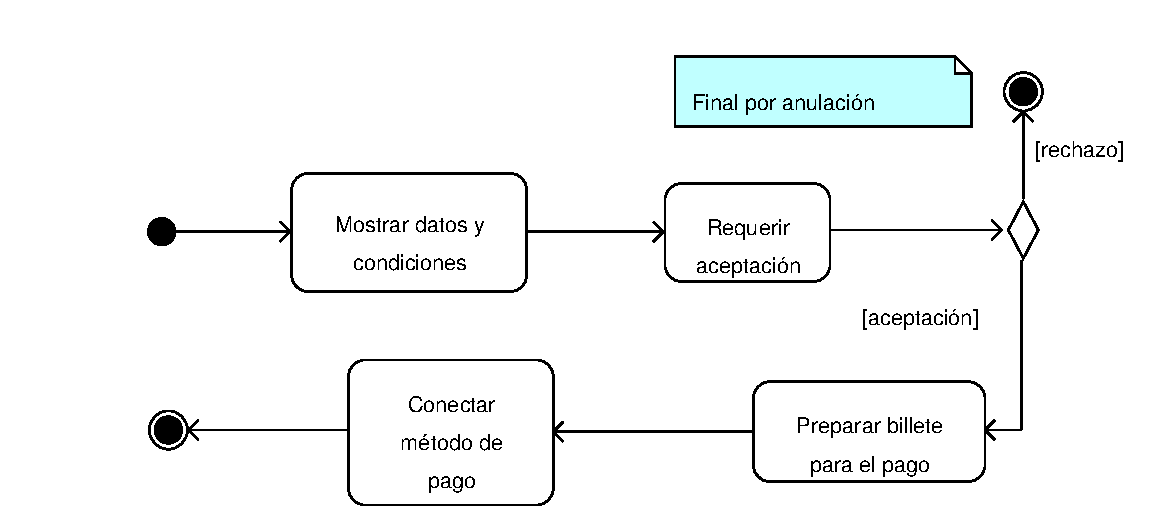
\includegraphics[scale=.76]{analisis/diagramas/da_iniciarpagobilletes.pdf}
				\end{center}

				El caso de uso {\itshape Iniciar pago billetes} se encarga de conectar el caso de uso {\itshape Comprar billete} con los diferentes métodos de pago.

				Al sólo haber desarrollado un método de pago el flujo de comportamiento queda de la siguiente forma: se muestran los datos y condiciones de la compra y el pago y se requiere la aceptación del usuario. Si el usuario rechaza las condiciones se aborta la operación. Si las acepta se prepara el billete para el pago y se conecta con el método de pago correspondiente.

			\subsubsection{Mostrar ofertas}
				\begin{center}
				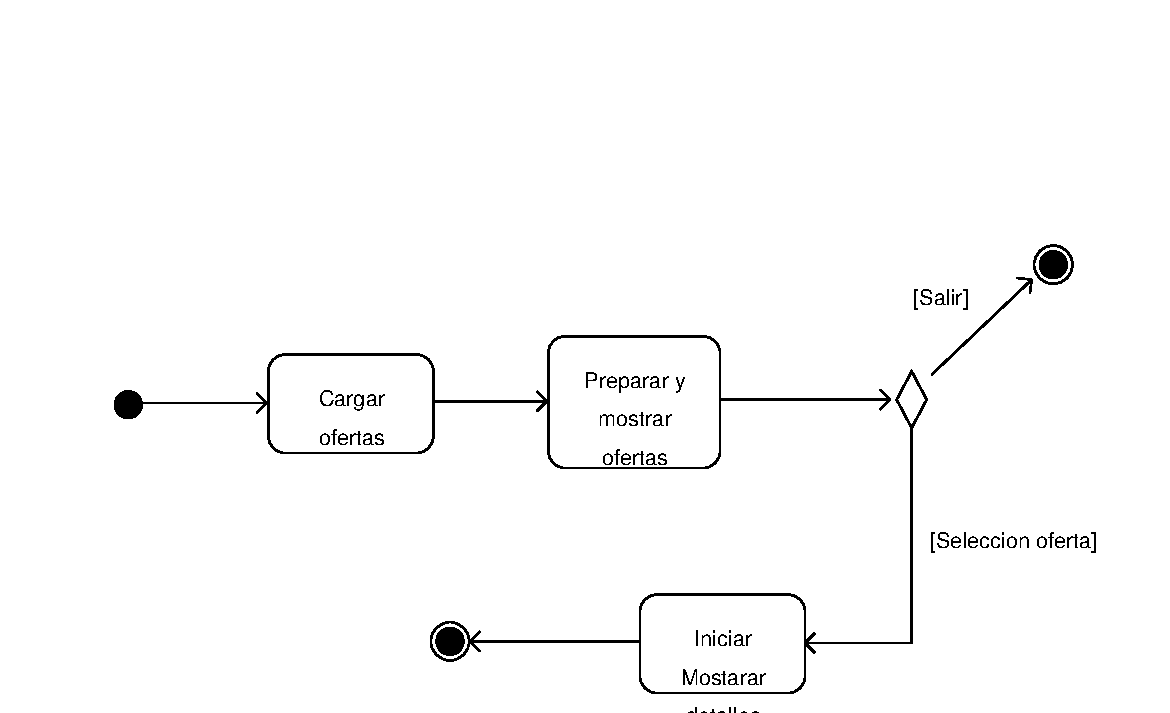
\includegraphics[scale=.72]{analisis/diagramas/da_mostrarofertas.pdf}
				\end{center}
				El caso de uso {\itshape Mostrar ofertas} permite visualizar todas las ofertas disponibles en el sistema. 
				El sistema empieza cargando todas las ofertas para preparar toda la información. Posteriormente se muestran las ofertas. Una vez aquí, el usuario puede decidir si salir de la muestra de ofertas, volver al menú principal y terminar este caso de uso, o seleccionar una oferta y redireccionar al inicio de mostrar una oferta.

			\subsubsection{Realizar pago con tarjeta}
				\begin{center}
					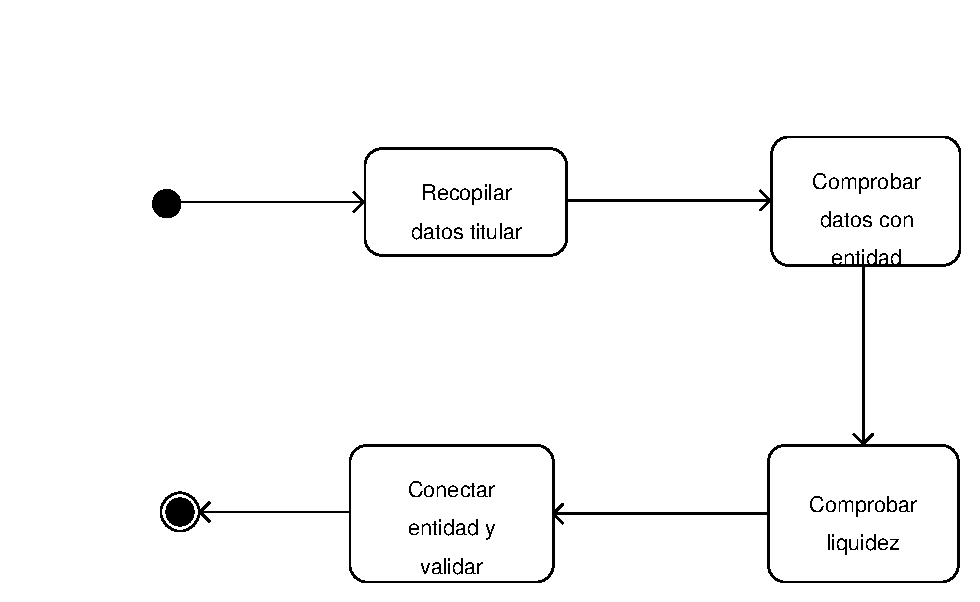
\includegraphics[scale=.7]{analisis/diagramas/da_pagotarjeta.pdf}
				\end{center}
				El caso de uso {\itshape Realizar pago con tarjeta} tiene la funcionalidad de terminar el proceso de pagado del pedido, pidiendo al usuario los datos del titular y número de cuenta. Después, realiza una comprobación de dichos datos conectando con la entidad financiera correspondiente para que pueda validar y comprobar la liquidez de la cuenta. Posteriormente carga el pago y pone la compra como finalizada, ya que en nuestra aplicación siempre va a ser correcto el pago pues no hay ningún tipo de conexión externo ni comprobaciones complicadas.
				
			\subsubsection{Presentar reclamación}
				\begin{center}
					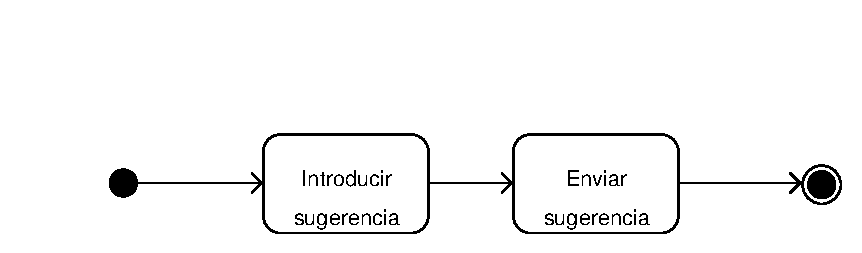
\includegraphics[scale=.82]{analisis/diagramas/da_presentarreclamacion.pdf}
				\end{center}
				Este caso de uso se basa en recoger una sugerencia introducida por un usuario para así después procesarla y enviarla al sistema de la base de datos de la compañía.

			\subsubsection{Registrarse}
				\begin{center}
					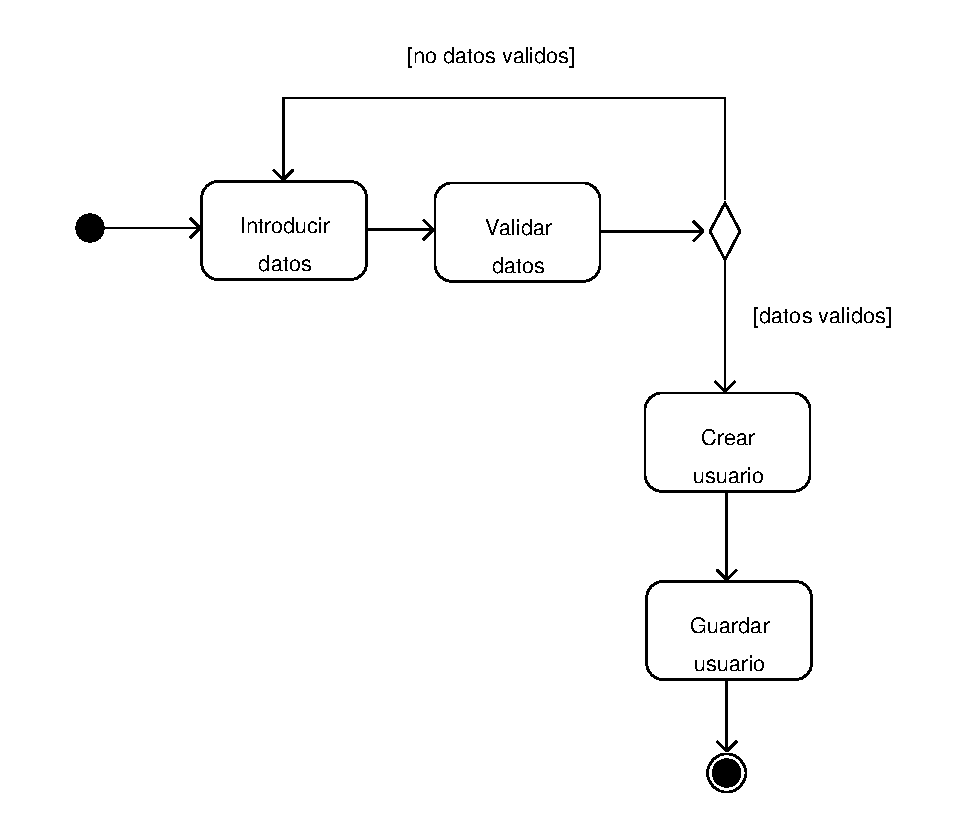
\includegraphics[scale=.8]{analisis/diagramas/da_registrarse.pdf}
				\end{center}
				
				El caso de uso {\itshape Registrarse} es el que permite registrar y guardar usuarios en el sistema. 
				Comienza cuando el cliente introduce sus datos y los valida, pudiendo ser estos no válidos y se volvería a pedir al usuario los datos, o pudiendo ser válidos y seguir el proceso con normalidad. Si es así, se creará un nuevo usuario y el sistema lo procesará para guardarlo en la base de datos.

			\subsubsection{Restablecer contraseña}
				\begin{center}
					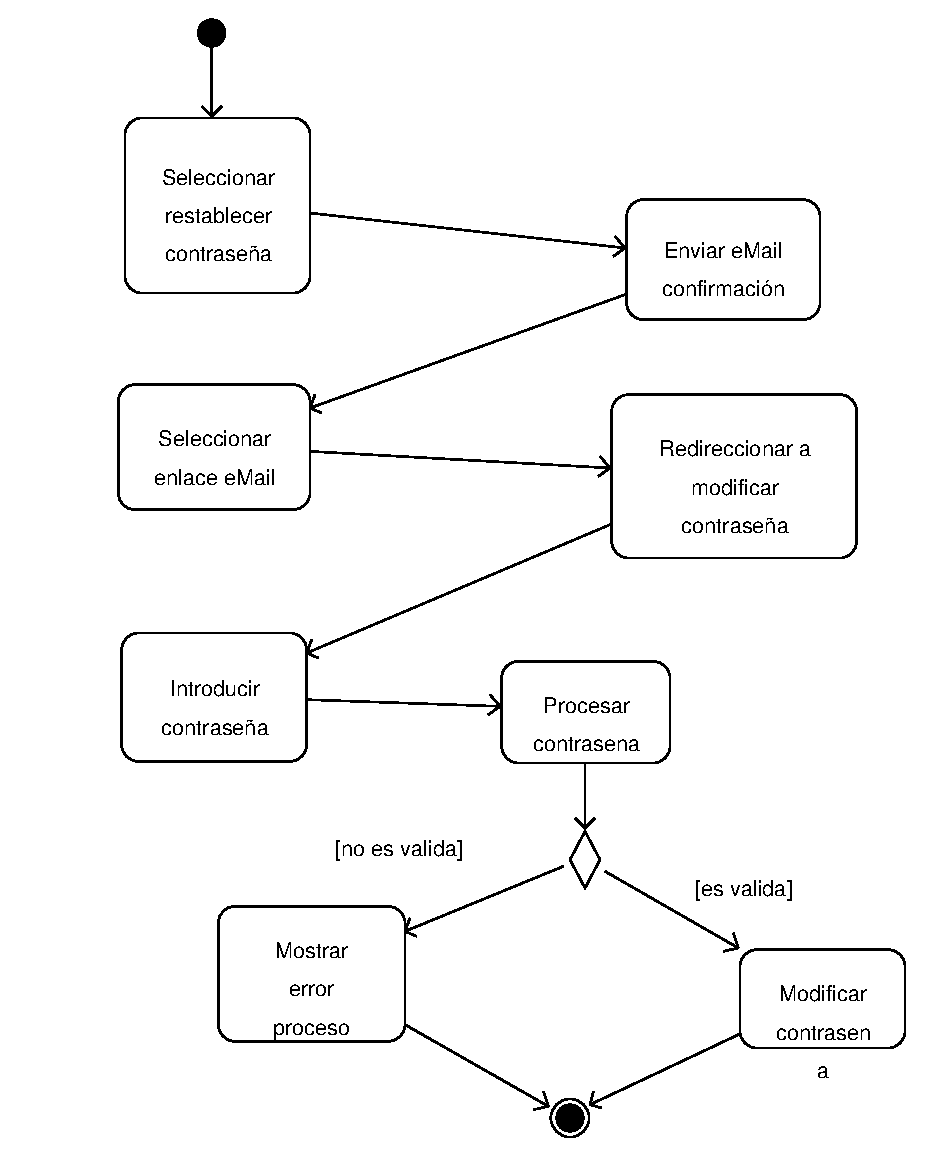
\includegraphics[scale=.8]{analisis/diagramas/da_restablecercontrasena.pdf}
				\end{center}
				Este caso de uso permitirá al usuario restablecer la contraseña. El sistema envía al usuario a través del servidor un eMail de confirmación de restablecimiento de la contraseña, para que el usuario seleccione el mail, el servidor web lo redireccione al lugar donde el usuario puede cambiar sus datos. Este introduce la contraseña y se procesa para su validación. Si es válida, se modifica la contraseña, y si no es válida se muestra un mensaje de error.
				
			\subsubsection{Ver información de vuelo contratado}
				\begin{center}
					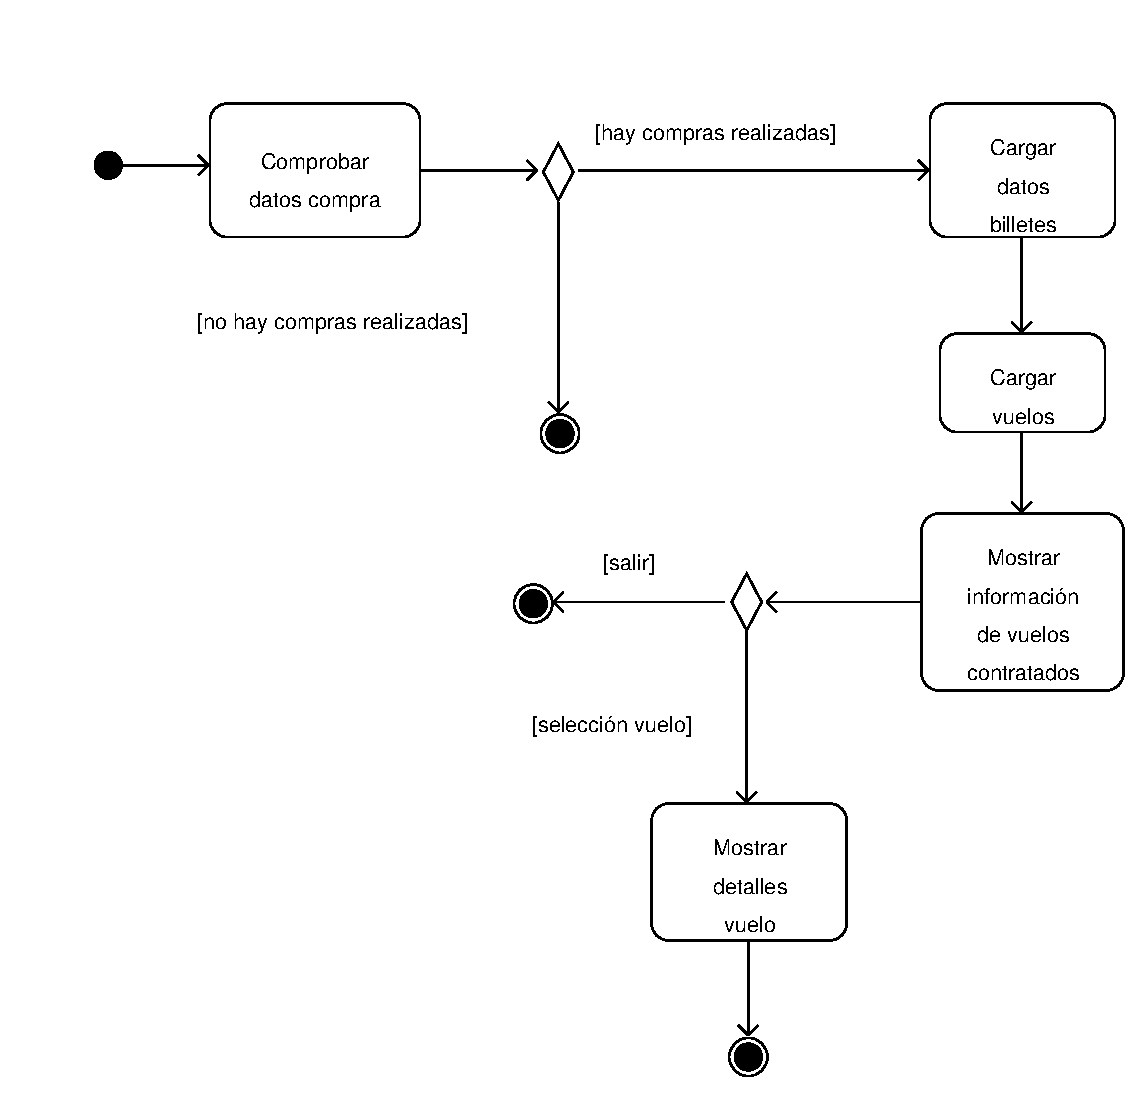
\includegraphics[scale=.8]{analisis/diagramas/da_verinfovuelocontratado.pdf}
				\end{center}
				En este caso de uso se comienza comprobando los datos de las compras realizadas. Se evalúa si dichas compras existen, pues en caso negativo la operación termina. En el otro caso, se cargan los datos de los billetes y los vuelos para poder posteriormente mostrar la información de los vuelos contratados. Una vez aquí, si el usuario no selecciona ningún vuelo, el proceso termina. Si selecciona un vuelo, se muestran los detalles del vuelo pulsado y finaliza el caso de uso.

	\newpage
	
	% -- Análisis
\begin{landscape}
	\section{Análisis}
		\subsection{Diagrama de paquetes}
		\vfill
		\begin{center}
			\hspace*{-.5cm}
			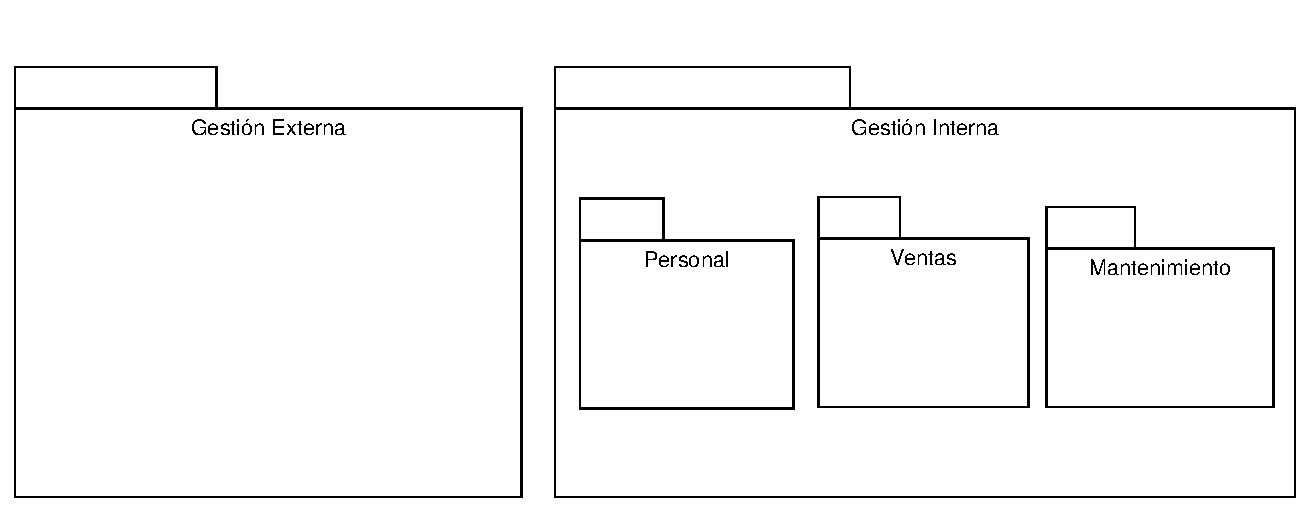
\includegraphics[scale=1]{analisis/diagramas/paquetes.pdf}
		\end{center}
		\vfill
\end{landscape}
		\subsection{Diagramas de comunicación}
			\subsubsection{Acceder web}
				\begin{center}
					\includegraphics[scale=.75]{analisis/diagramas/accederweb.pdf}
				\end{center}

				A través de la interfaz {\itshape PáginaAcceso} el usuario introduce sus datos de identificación personal (a saber, su nombre de usuario y contraseña). El sistema busca en la base de datos de usuarios registrados (representada en {\itshape RegistroUsuarios}) un usuario que se corresponda con los datos aportados. Si fuese necesario se cargarían las preferencias personales del usuario. Al finalizar la secuencia el usuario tiene una sesión activa que le da acceso a otras características de la aplicación.

				La entidad {\itshape Usuario} representa a un usuario registrado de la página web, que no es necesariamente un cliente. La entidad lo representa por medio de unos datos personales básicos como puede ser un identificador único, una clave secreta y una dirección de contacto.


			\subsubsection{Comprar billete}
				\begin{center}
					\includegraphics[scale=.72]{analisis/diagramas/comprarbillete.pdf}
				\end{center}
					
					La interfaz  de {\itshape Comprar billete} lleva a la página de {\itshape Datos de compra} en la que el usuario introduce sus datos personales para generar el billete. A continuación, se comprueban los datos y si son correctos nos lleva a la interfaz de {\itshape Iniciar Pago de Billete}.

					La entidad {\itshape Billete} respresenta un billete de un determinado vuelo. Un biillete queda determinado por un vuelo, un pasajero, un precio y una clase (que puede ser:  business, turista, grupos, acuerdos especiales y touroperador).


			\subsubsection{Consultar oferta}
				\begin{center}
					\includegraphics[scale=.85]{analisis/diagramas/consultaroferta.pdf}
				\end{center}
					
					El caso de uso {\itshape Consultar Oferta} recibe una oferta de {\itshape Mostrar ofertas}. Se procede a cargar los datos (nombre, destino, decuento y condiciones para acceder a dicha oferta) y a mostrar dicha oferta al usuario.
					La entidad {\itshape Oferta} representa a una oferta del catálogo de ofertas.

			\subsubsection{Consultar vuelos}
				\begin{center}
					\includegraphics[scale=.71]{analisis/diagramas/consultarvuelos.pdf}
				\end{center}
			
			\subsubsection{Editar datos personales}
				\begin{center}
					\includegraphics[scale=.86]{analisis/diagramas/editardatospersonales.pdf}
				\end{center}


			\subsubsection{Iniciar pago billetes}
				\begin{center}
					\includegraphics[scale=.76]{analisis/diagramas/iniciarpagobilletes.pdf}
				\end{center}

					El caso de uso {\itshape Iniciar Pago de Billetes} recibe los datos de un billete de vuelo (en el diseño se ha generalizado a una asociación de billetes denominada {\itshape compra}) y tras mostrar una página de confirmación al usuario de las condiciones de la misma, se procede a la confección del billete y a la selección del método de pago\footnote{Realmente sólo se ha desarrollado un método de pago (\nameref{ana:tarjeta}) por lo que la selección del método se hace automáticamente.}. Finalmente el caso de uso se comunica con el método de pago seleccionado (a través de una interfaz conveniente) para continuar la operación.

			\subsubsection{Mostrar ofertas}
				\begin{center}
					\includegraphics[scale=.72]{analisis/diagramas/mostrarofertas.pdf}
				\end{center}

			\subsubsection{Realizar pago con tarjeta} \label{ana:tarjeta}
				\begin{center}
					\includegraphics[scale=.7]{analisis/diagramas/pagotarjeta.pdf}
				\end{center}

			\subsubsection{Presentar reclamación}
				\begin{center}
					\includegraphics[scale=.82]{analisis/diagramas/presentarreclamacion.pdf}
				\end{center}

					A través de la interfaz {\itshape PáginaSugerencias} el usuario envía una sugerencia y se prodece al envío de la misma.

			\subsubsection{Registrarse}
				\begin{center}
					\includegraphics[scale=.8]{analisis/diagramas/registrarse.pdf}
				\end{center}

					A través de la interfaz {\itshape Registrarse} el usuario introduce sus datos personales (nombre, apellidos, correo y contraseña) y se prodece a la comprobación de los mismos. Si todo ha ido correctamente se crea un nuevo usuario con esos datos y queda registrado.

			\subsubsection{Restablecer contraseña}
				\begin{center}
					\includegraphics[scale=.77]{analisis/diagramas/restablecercontrasena.pdf}
				\end{center}


					El caso de uso {\itshape Restablecer contraseña} consiste en enviar un email  al correo asociado del usuario. En ese correo el usuario introducirá la nueva contraseña, que será comprobada y modificada en la base de datos del usuario.
			\subsubsection{Ver información de vuelo contratado}
				\begin{center}
					\includegraphics[scale=.8]{analisis/diagramas/verinfovuelocontratado.pdf}
				\end{center}

					A través de la interfaz {\itshape PáginaVueloSeleccionado} se carga la información del vuelo seleccionado en  {\itshape Consultar vuelos}. Una vez que se ha cargado la información se muestran los detalles del vuelo seleccionado, a saber: el aeropuerto de origen, la fecha de salida, el aeropuerto de destino, la fecha de llegada, el número de vuelo, el número de pasajeros, el número de escalas y el precio del billete.

\begin{landscape}
		\subsection{Diagrama de clases}
			\begin{center}
				\vspace{2cm}
				\hspace{-2cm}
				\includegraphics[scale=1]{analisis/diagramas/diagramaclases.pdf}
			\end{center}	
\end{landscape}
\begin{landscape}
			\begin{center}
				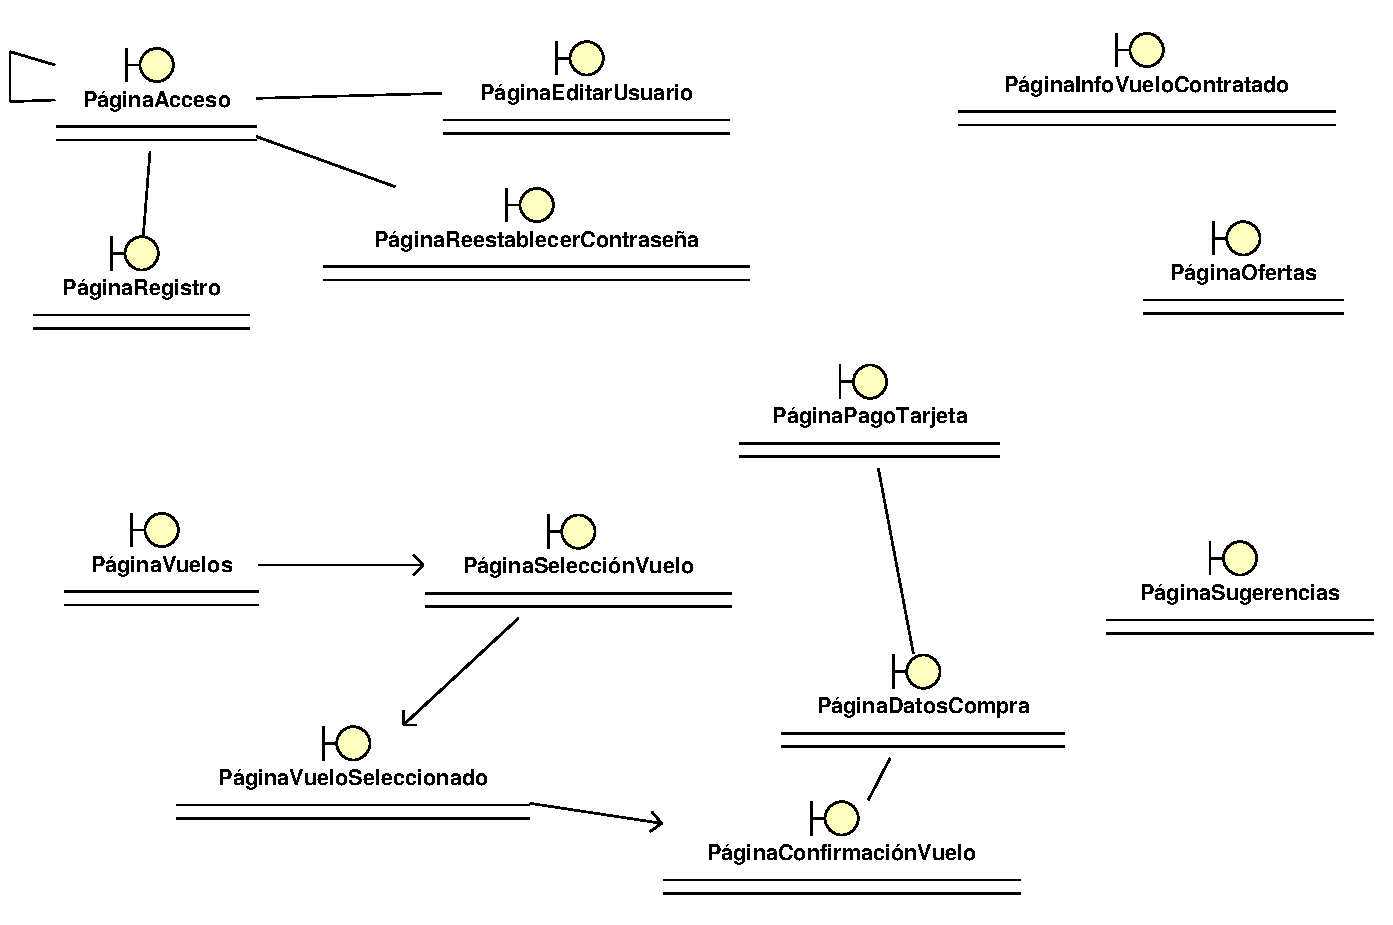
\includegraphics[scale=1]{analisis/diagramas/sitioweb.pdf}
			\end{center}
\end{landscape}
	\newpage

	% -- Diseño
	\section{Diseño}
		\subsection{Introducción}
			La interfaz de gestión externa se ha implementado como una aplicación gráfica de escritorio utilizando la biblioteca gráfica {\itshape Swing} del lenguaje de programación {\itshape Java}.

			Por un lado se encuentran las clases representantes de objetos del dominio (como \textit{Vuelo}, \textit{Billete}, \textit{Pasajero} \ldots) y otras clases artificiales que realizan funciones necesarias para la aplicación (siguiendo el criterio GRASP de la \textit{fabricación pura}), especialmente en lo concerniente al manejo y la persistencia de los datos.

			Otra parte de la aplicación la componen las clases relacionadas con la comunicación con el usuario por medio de la interfaz gráfica. El modelo consiste en una \textit{VentanaPrincipal} compuesta por varias clases auxiliares que contiene un marco intercambiable donde se muestran las diferentes pantallas correspondientes a los diferentes casos de uso. Al tratarse de la interfaz externa, la aplicación se ha diseñado con cierta apariencia de página web.

			Para la puesta en práctica del almacenamiento de los datos se ha utilizado la \textit{serialización} de Java con aquellos objetos que así lo requieren.

		\subsection{Diagramas de secuencia}
			\subsubsection{Acceder web}
				\begin{center}
					\includegraphics[scale=.7]{diseno/diagramas/accederweb.pdf}
				\end{center}

			\subsubsection{Comprar billete}
				\begin{center}
					\includegraphics[scale=.67]{diseno/diagramas/comprarbillete.pdf}
				\end{center}

			\subsubsection{Consultar oferta}
				\begin{center}
					\includegraphics[scale=.7]{diseno/diagramas/consultaroferta.pdf}
				\end{center}

			\subsubsection{Consultar vuelos}
				\begin{center}
					\includegraphics[scale=.5]{diseno/diagramas/consultarvuelos.pdf}
				\end{center}

				La pantalla {\itshape PantallaConsultaVuelos} permite al usuario buscar vuelos por diferentes criterios (aeropuerto de salida, aeropuerto de llegada, fecha de salida, fecha de llegada, \ldots) y muestra los resultados de las búsquedas con la información básica que les corresponde. El usuario puede seleccionar una de las apariciones para ver una vista detallada del vuelo, con la información completa y poder desde allí acceder a la compra del billete.

				{\itshape GestorVuelos} representa un administrador de vuelos que permite obtener listas filtradas de entre los disponibles por medio de los criterios especificados.
			
			\subsubsection{Editar datos personales}
				\begin{center}
					\includegraphics[scale=.6]{diseno/diagramas/editardatospersonales.pdf}
				\end{center}


			\subsubsection{Iniciar pago billetes}
				\begin{center}
					\includegraphics[scale=.6]{diseno/diagramas/iniciarpagobilletes.pdf}
				\end{center}

			\subsubsection{Mostrar ofertas}
				\begin{center}
					\includegraphics[scale=.7]{diseno/diagramas/mostrarofertas.pdf}
				\end{center}

			\subsubsection{Realizar pago con tarjeta}
				\begin{center}
					\includegraphics[scale=.7]{diseno/diagramas/pagotarjeta.pdf}
				\end{center}

			\subsubsection{Presentar reclamación}
				\begin{center}
					\includegraphics[scale=.7]{diseno/diagramas/presentarreclamacion.pdf}
				\end{center}

				Por medio de la pantalla {\itshape PantallaSugerencias} el usuario expone su sugerencia, incluyendo con ella --de forma opcional-- su nombre y una dirección de contacto donde recibir respuesta. {\itshape PantallaSugerencias} construye una sugerencia ({\itshape recl}) con los datos aportados. La operación de construcción de {\itshape Sugerencia} puede dar lugar a errores si el mensaje de sugerencia es vacío o la dirección de correo electrónico de contacto no se ajusta al formato. Si no se producen esos hechos habrá construida una {\itshape Sugerencia} válida que será enviada a la compañía por medio de la clase {\itshape GestorSugerencias} que devolverá un número identificativo del registro que deberá ser mostrado al usuario para futuras alegaciones.

			\subsubsection{Registrarse}
				\begin{center}
					\includegraphics[scale=.5]{diseno/diagramas/registrarse.pdf}
				\end{center}

			\subsubsection{Restablecer contraseña}
				\begin{center}
					\includegraphics[scale=.6]{diseno/diagramas/restablecercontrasena.pdf}
				\end{center}

			\subsubsection{Ver información de vuelo contratado}
				\begin{center}
					\includegraphics[scale=.7]{diseno/diagramas/verinfovuelocontratado.pdf}
				\end{center}
			
		\subsection{Diagrama de clases}
			\begin{center}
				\hspace{-2cm}
				\includegraphics[scale=.57]{diseno/diagramas/diagramaclases.pdf}
			\end{center}

		\subsection{Aplicación de patrones de diseño}
En el diseño de esta aplicación \software se han utilizado de forma intencionada o casual algunos patrones de diseño orientado a objetos que han sido explicados en clase.

		Para la asignación de responsabilidades y relaciones a las clases se ha intentado aplicar el patrón \textit{Experto}, reducir el acoplamiento y 	mantener una alta cohesión.

		A lo largo de toda la aplicación se puede observar el patrón GRASP denominado \textit{Polimorfismo}. Los ejemplos más notables son los métodos de pago (\textit{MetodoPago}) y las \textit{Pantalla}s asociadas a los casos de uso en la interfaz gráfica, casos que también son ejemplos del patrón \textit{Puente}.

		En la interfaz gráfica se recurre también al patrón \textit{Observer}, bien organizado por el propio \textit{Swing} (\textit{Java}), bien implementado para usos particulares.

		En las clases asociadas a la persistencia de los datos (en teoría, la comunicación con la base de datos; en la práctica, el control de archivos persistentes) se pone en práctica el modelo \textit{Solitario}, ya que es especialmente conveniente por la unicidad de la fuente de datos y la conveniencia de utilizar operaciones sobre instancias en lugar de métodos estáticos (por ejemplo la segunda posibilidad restringe las facilidades de serialización).

		Una interpretación del patrón \textit{Visitante} es utilizada en los criterios de búsqueda a los que se les hace recorrer una lista de candidatos, comprobando en cada uno de ellos si cumplen los criterios establecidos.


\end{document}
